\documentclass[../rzero]{subfiles}
\begin{document}
\chapter{Monopole Gravitational Waves}\label{monopoleGravitationalWavesChapter}

\begin{chapquote}{Standard Model Physicist, \textit{Astro 498\cite{Astronomy498}}}
``Now consider gravitational radiation. Let the mass-energy density be $\rho(r)$. The monopole moment is $\int \rho(\mathbf{r}) d^3 r$, which is simply the total mass-energy. This is constant, so there cannot be monopolar gravitational radiation.''
\end{chapquote}

\section{Monopole Waves}
Monopole Waves are waves that emanate spherically from a source. Due to symmetry, they can really only be pressure, also known as longitudinal waves. The typical example is a spherical speaker (who has spherical speakers? Is it 1974 or something?). The sound (sound is a pressure wave) goes in all directions and each wave crest forms a spherical pattern, moving away from the speaker at the speed of sound. That is how acoustic monopole waves work. Let's look at General Relativity now.

\section{They Can't Exist}
One of the most famous theorems of General Relativity is Birkhoff's Theorem\cite{Birkhoff1923}. It's clear, the gravitational field outside a spherical mass is always exactly the static Schwarschild field. So with that big word static in there, it seems there cannot be and monopole gravitational waves. Case closed. 

One can, however, make (an almost trivial) 'dragged along' monopole gravitational wave by imagining a typical supernova explosion, with an unlucky observation spacecraft orbiting around it. The basics are depicted in figure (\ref{monopoleFigure}) In a supernova a large amount of energy is emitted as neutrinos as the first step, about 1/1000 of a solar mass worth of energy. The spaceship has no neutrino detector on board, but can of course observe its own motion accurately. It will notice the central mass drop as the (undetected) neutrinos pass by. This wave (not self supported), is a monopole $p-wave$, it's spherically symmetric, and will resize a ring of beads in manner so as to allow the extraction of energy (Feynman's criteria). It doesn't violate Birkhoff's Theorem, the gravitational field always looks spherical, and describes the mass - energy still left inside the position of the spacecraft.

\begin{figure}\label{monopoleFigure}
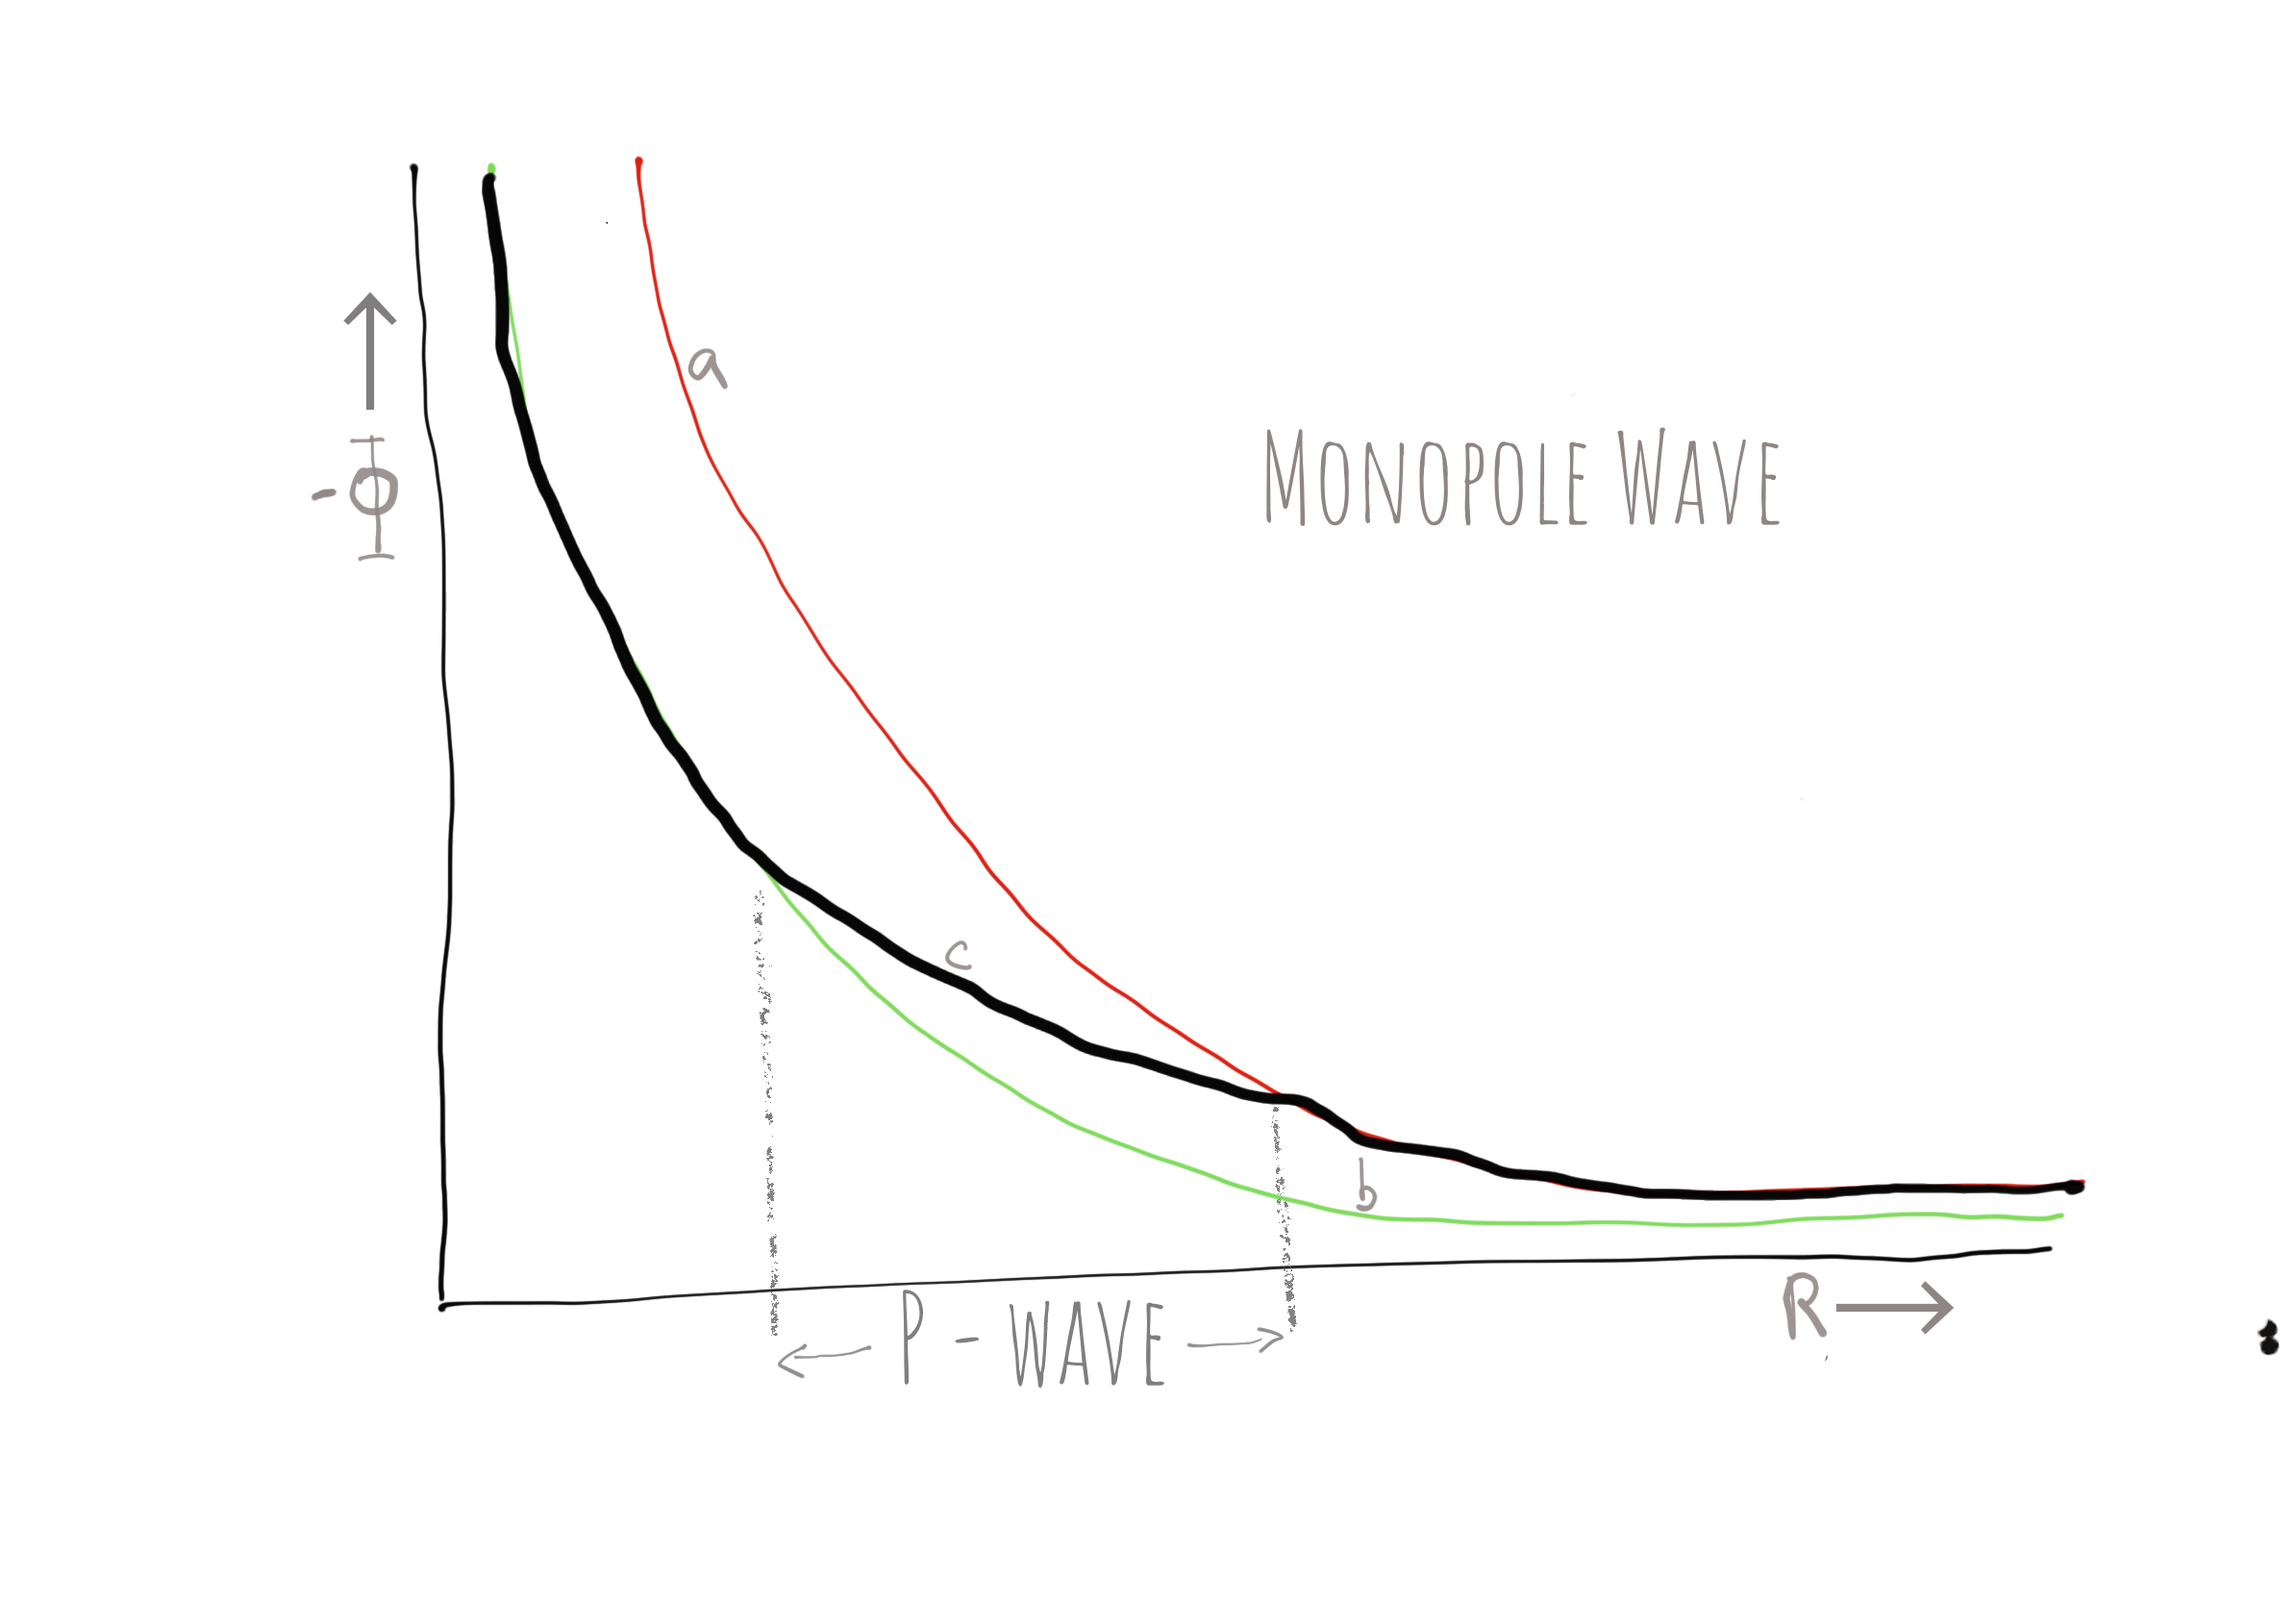
\includegraphics[width=\textwidth]{chapters/images/monopole.png}
\caption{Monopole Wave: Birkhoff's theorem holds even for a dynamic situation as, for instance discussed in the text. The left axis is the negative of the gravitational potential, bottom axis is radius. Curve $a$ is for a large mass, $b$ for a small mass, and $c$ for the actual physics. The region shown by the label $P - Wave$ is the location of the moving monopole gravitational wave.}
\end{figure}


\subsection{Vacuum solution}
Another example of this phenomenon is obtained by looking at a LIGO\cite{abbott2016gw150914} event using the vacuum Einstein Equations $R_{\mu\nu} = 0$(equation \ref{vacuumEquation} in the intro again). In that spectacular 2015 $GW150914$ LIGO event, about 3 solar masses of energy were emitted. It's interesting to think about the 3 solar mass monopole wave that must have accompanied it as being a part of the pure vacuum field equations, after all the entire $GW150914$ event took place in an Einstein vacuum region.   

\textit{But the Einstein equations don't automatically include the energy of the gravitational field itself.} One has to 'cheat' and move the gravitational waves to the right side of the equation (into T) to get anything to work at all. Which likely isn't good. 

So people naturally look for solutions to this problem. \cite{dereliEnergyMomentumDensityGravitational2004}  
\begin{quotation}
	Thus non-trivial gravitational fields that satisfy the Einstein field equations with T = 0 have no covariantly defined mass-energy or momentum densities associated with them.
\end{quotation}

It may be that the Einstein theory of General Relativity is missing something!\cite{08092323EnergyMomentumGravitational}. See chapter \ref{energyGeneralRelativityChapter} - where I look at this in depth. 

\section{Energy argument for their existence}
In this chapter, instead of looking at how to perhaps modify Einstein's General Relativity, I look at an energy based argument for the existence of monopole gravitational waves. I think the rational for independent (non dragged - along) monopole waves is strong, and I don't want to muddy the waters by looking at one psuedo tensor or other approach.  

\subsection{Brown \& York and Lynden-Bell \& Katz}
The fact that Einstein's equations don't describe energy in the actual field just \textit{feels} wrong. To deal with this feeling, physicists have come up with some ways to think about the energy in a gravitational field. It's called 'quasi-local' energy. In most papers on quasi local energy, the authors don't discuss ways of modifying the Einstein field equations to take this quasi local energy into account, they 'merely' come up with expressions that describe energy in the gravitational field. 

So my plan is as follows: I look at the expressions for gravitational energy in the field from Brown and York\cite{Brown1993}, and Lynden-Bell Katz\cite{lyndenbell1985}. 

Looking again at figure \label{monopoleFigure}, this time instead of a accompanying burst of energy (like the supernova neutrinos or the gravtitational waves of a LIGO event), I will try and look at the excess energy in the 'P - wave' zone in the image, and imagine it moving, either outward or inward. 

Consider a spherical area of Minkowski (flat) geometry (Figure \ref{monopoleEnergy}). The energy in this interior area is zero. Outside of this region is a region of vacuum gravitational energy, in the form of a Schwarzschild metric, truncated at the boundary, say at $\bar r$ . As per Birkhoff's theorem, we really have no choice, this exterior region must look like a black hole of mass $M$ from the outside. See Vishwakarma\cite{vishwakarmaMysteriesRikNovel2014} for details on the reality of energy in the gravitational field. 

\begin{figure}\label{monopoleEnergy}
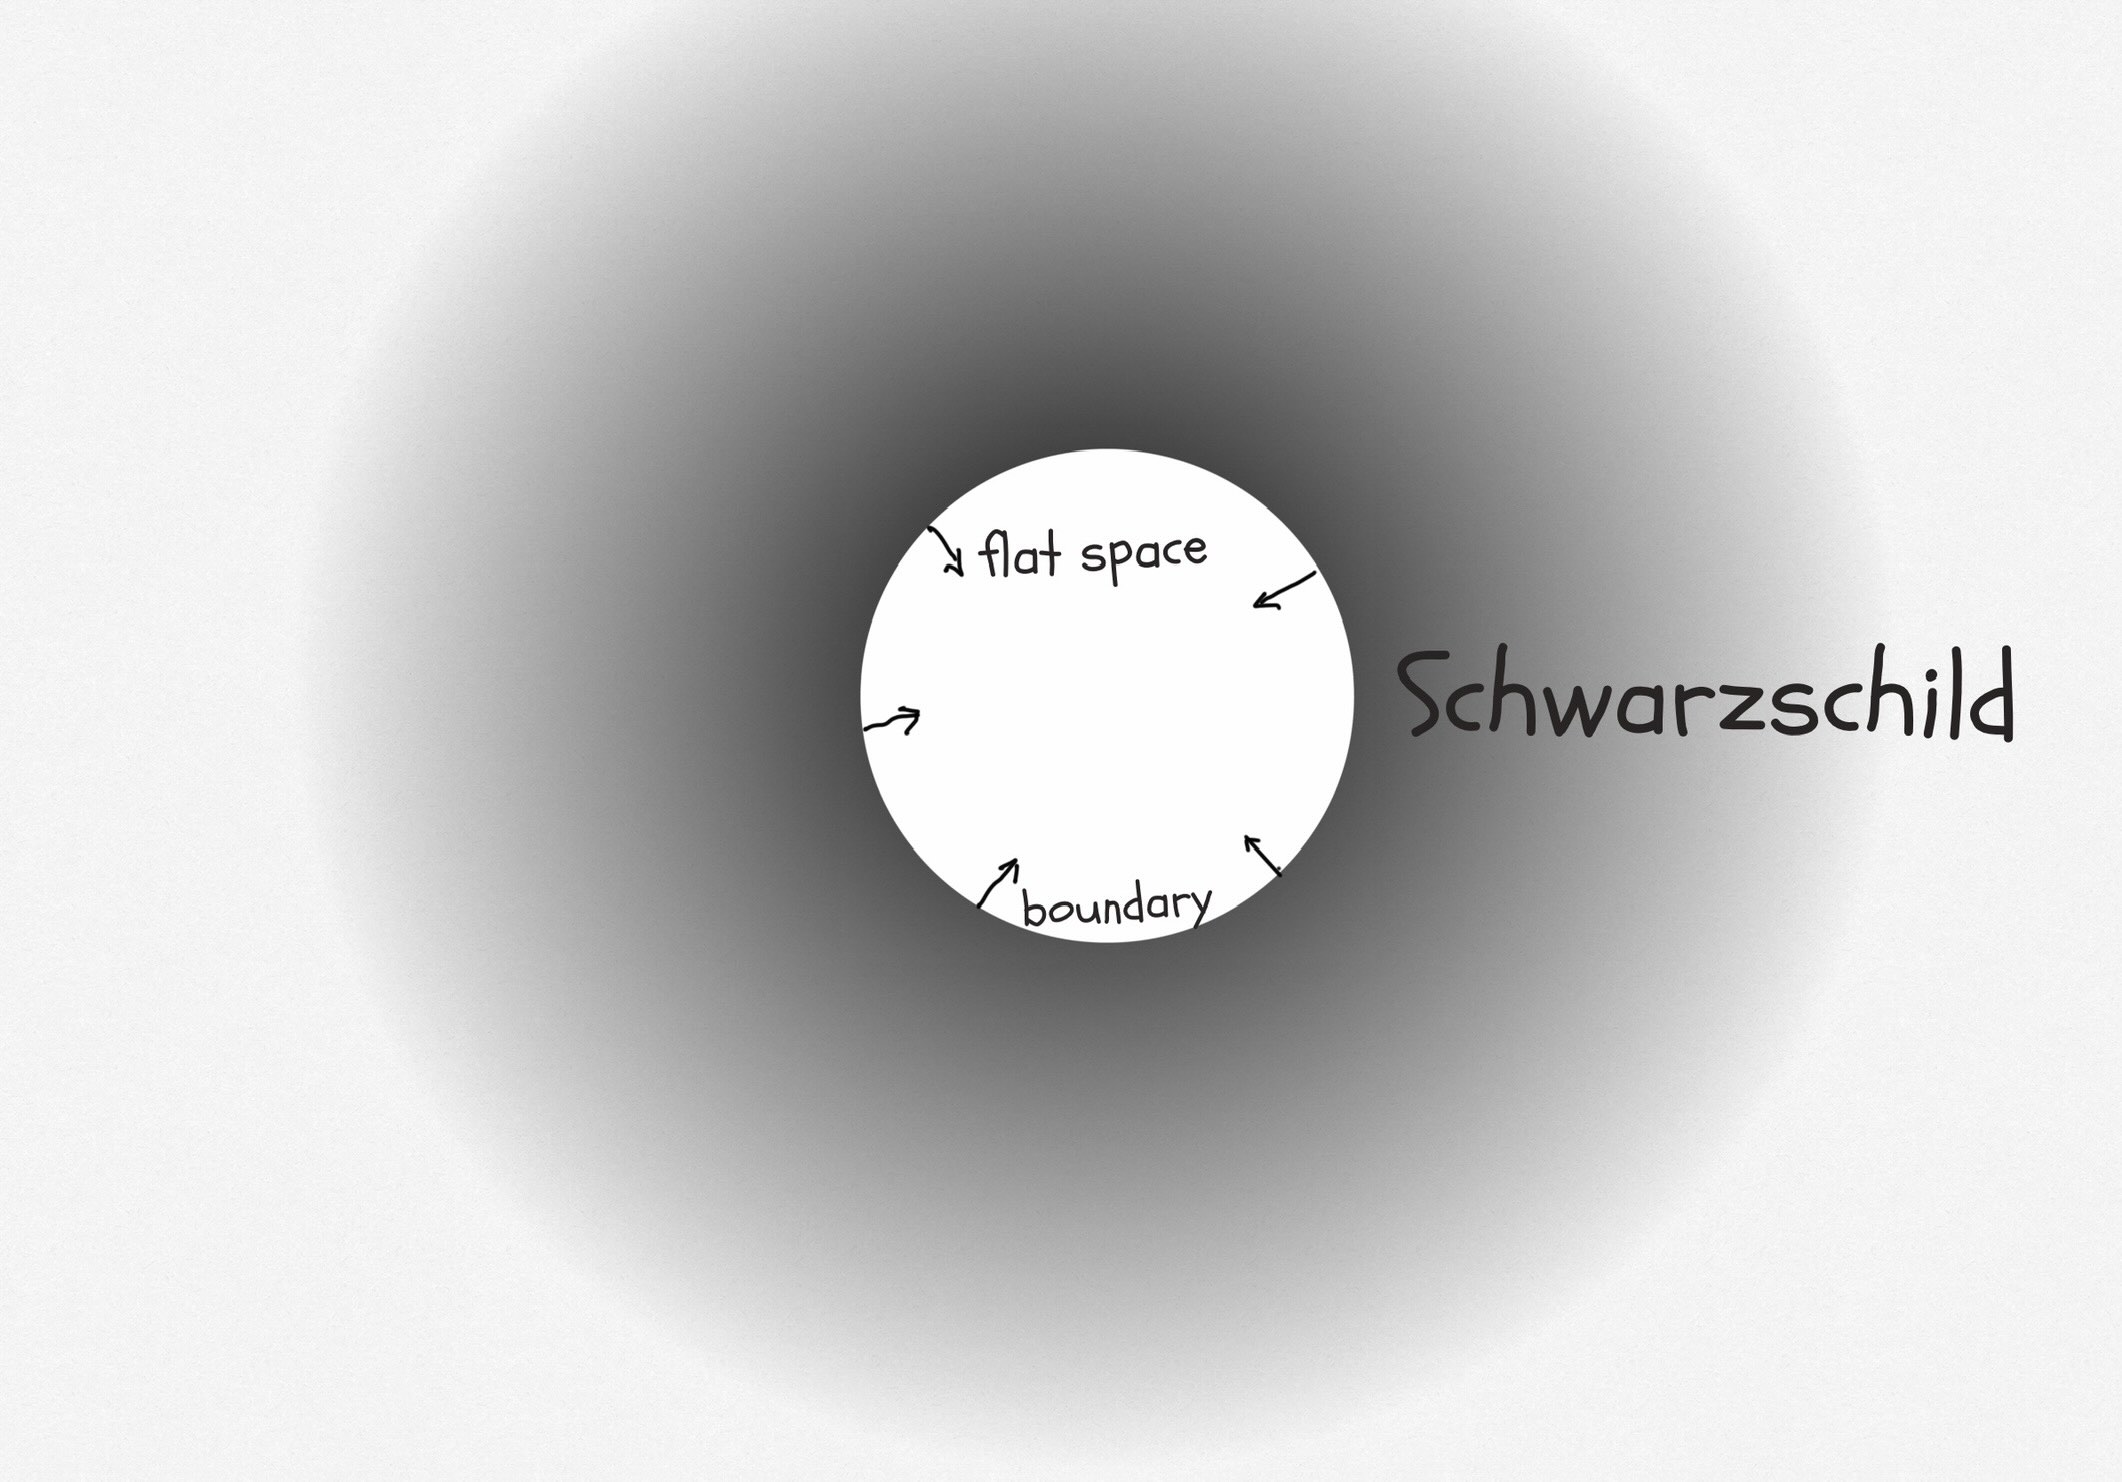
\includegraphics[width=\textwidth]{chapters/images/monopole-energy.jpg}
\caption{Monopole Energy: In the outer region there is a Schwarzschild metric, which is impinging on a spherical region of flat space. We will find that the boundary must be rapidly moving to satisfy energy conservation.}
\end{figure}


Now let's consider the gravitational field energy in this system. From Lynden-Bell and Katz\cite{lyndenbell1985}, the field energy outside of $\bar r$ (in isotropic coordinates, hence the use of the notation $\bar r$) is 

\begin{equation} \label{energyoutsideR}
 GM^2/2 \bar r .
\end{equation}

We note that at the horizon, in isotropic coordinates, the radius is $ \bar r = GM/2 $, so for a complete, \lq normal\rq\ black hole we see all the mass of the black hole is in the field. That's the basic idea of the Brown-York energy density.

However, with our \lq hollowed out\rq\ Schwarzschild solution, there will be an mass/energy shortfall, for any $\bar r$ the  - where is this energy? While energy can get tricky in general relativity, nothing is stopping us from starting with the flat region being of a large radius $\bar r$ to put general relativity into an almost linear regime, where energy conservation is simple. We assume that this missing energy is kinetic energy - that the boundary is rapidly moving (gravitational fields can also carry kinetic energy). Thus the total energy in the entire diagram (inner flat + outer) region is:

\begin{equation} \label{energyBalanceEqn}
 M = GM^2/2 \bar r + K.E.
\end{equation}

Where the LHS $M$ comes from use of Birkhoff's theroem. For K.E. we can use either the Lorentz or Newtonian formulas. 

\subsubsection{Using Newtonian Kinetic Energy}

Using Newtonian mechanics, rearranging (\ref{energyBalanceEqn}), and assuming that the effective moving mass is a function of radius, $m(r)$,

\begin{equation}\label{newtonBalance}
 \frac{1}{2}m(r)v^2 = M - GM^2/2 \bar r , 
\end{equation}

What is this dynamic - moving mass $ m(r) $? We note that most of the mass is near the boundary area since the Brown-York energy is mostly all near the inner surface, so   $m(r) \approx GM^2/2 \bar r $. Making the substitution in to (\ref{newtonBalance}), and solving for $v$ we get, still in isotropic coords,

\begin{equation}
 v = 2 \sqrt{\frac{\bar r}{G M} - \frac{1}{2}},
\end{equation}

or in the more often used Scwharzchild coordinates,
\begin{equation}
 v = 2 \sqrt{\frac{r}{G M} - 2}.
\end{equation}
Thus, if the boundary is moving at $v$, we have energy conservation and Birkhoff's theorem works at any radius. It's obvious that the velocity could be positive or negative, so the pulse could be moving in or out. The calculated velocity here is greater than the speed of light (which is 1 here), except for close to the horizon. It's easy to calculate, and is often about $10^4c$ in places like earth bound labs and interstellar space. It seems to be frame dependent, too - since the speed depends on the (inverse of) the gravitational potential, $GM/r$, a global fact of the spacetime. 

For complicated spacetimes, such as on the surface of the earth, an approximate value of $v$ can be calculated by looking at the nearest masses and picking the slowest speed. (At earth's surface, remembering the GM for the earth is about a centimeter, and the earth is 6000km), 

\begin{equation}
 v_{earth} = 2 \sqrt{\frac{6000km}{1 cm} - 2} \ \approx 25000c .
\end{equation}
From the sun on earth:
\begin{equation}
 v_{sun} = 2 \sqrt{\frac{150e6km}{1 km} - 2} \ \approx 12000c .
\end{equation}

The reason, in our view, for taking the time to layout the Newtonian superluminal solution for this velocity is that the solution already violates the equivalence principle, perhaps implying a more Lorentzian viewpoint  of Einstein's Ether\cite{Einstein1920}. Namely that there is a special frame, and if there is, there must be Lorentz violation.  


\subsubsection{Relativisic KE}
Using a relativistic approach to the total energy, generically, 
\begin{equation}
 E = \frac{m}{\sqrt{1 - v^2}}.
\end{equation}

For the case here, we know the total energy is M, while the rest mass of the gravtiational field is $GM^2/2 \bar r $, so

\begin{equation}
 M = \frac{GM^2}{2 \bar r \sqrt{1 - v^2}}.
\end{equation}

Solving for v, 

\begin{equation}
 v = \sqrt{1 - \frac{G^2M^2}{4\bar r^2}}.
\end{equation}



This relativistic result seems to be the one to use, but it's still dependent to the gravitational potential, which is strange, and brings us back to a global potential dependent velocity. Which is why we are not sure that the relativistic speed is the one to use here. 

\section{Experimental Consequences}
Faster than light collapse



\section{Quantum Mechanics from General Relativity}
my theory


\section{Dark matter is quantum mechanics}
	Model is laid out 
\end{document}
